\section{Il contenuto}

Abbiamo dunque esaminato per bene la vetrina, siamo stati attirati dal ciò che ha esposto e abbiamo entrare nel negozio. È giunto dunque il momento di addentrarci in una pagina interna al sito ed analizzare come esso viene presentato.

Precisiamo fin da subito che articoli e guide sono presentate allo stesso modo, anzi, possono essere considerate fondamentalmente la stessa cosa.

\subsection{Struttura di una guida}

Prendiamo come esempio la guida Android, la quale mi è risultata molto utile nel momento in cui ho deciso di entrare in quel mondo. Ciò che vediamo a primo impatto è rappresentato dalla figura seguente:

\begin{figure}[H]
\centering
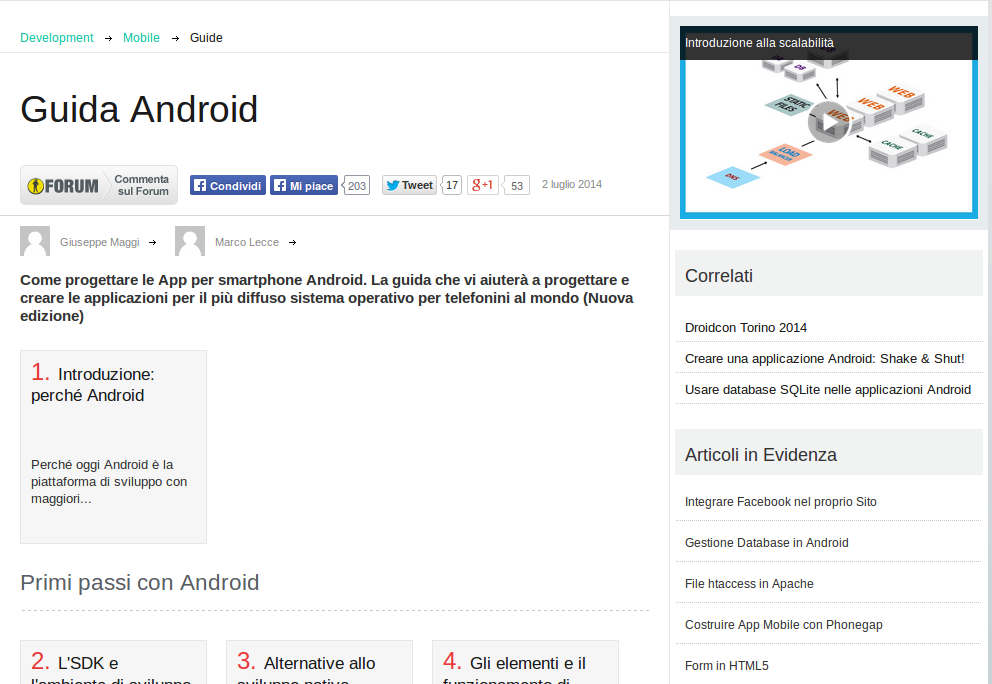
\includegraphics[width=120mm]{images/internal1.png}
\caption{Visualizzazione di una guida}
\end{figure}

\begin{figure}[H]
\centering
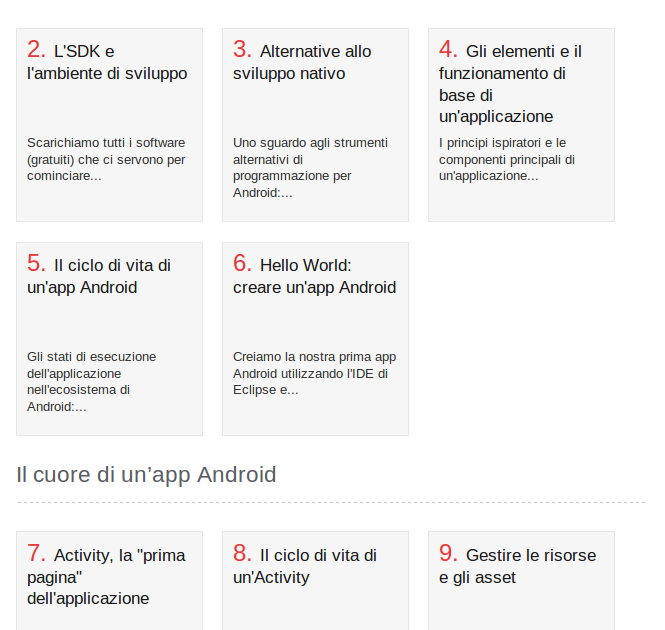
\includegraphics[width=120mm]{images/internal2.png}
\caption{Suddivisione in lezioni}
\end{figure}

Come possiamo vedere la guida è suddivisa in sezioni principali, le quali contengono un certo numero di \textbf{lezioni}. Le guide sono ben strutturate e gli argomenti sono in ordine crescente di complessità. Questo rende possibile navigare in maniera ipertestuale all'interno di una guida, dando la possibilità di scegliere determinati argomenti da approfondire. Le guide seguono certamente un filo logico e ciascuna lezione è collegata alla successiva, ma è comunque possibile partire da una lezione qualunque. La suddivisione a griglia permette ancora una volta una facile navigazione ed evita troppo scroll verticale all'utente.

Sulla \textbf{barra laterale} a destra sono inoltre presenti tutta una serie di link a guide o articoli correlati all'argomento o in evidenza, il che rende la navigazione più efficace ma, a mio modo di vedere, penalizza il contenuto, in quanto occupa troppo spazio e rischia di deviare troppo l'attenzione dell'utente.

\subsection{Breadcrumb}

Altra cosa interessante è la presenza dei \textbf{breadcrumb}, come risulta dalla figura seguente:

\begin{figure}[H]
\centering
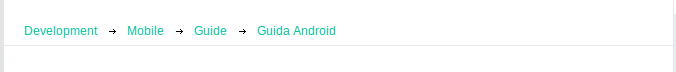
\includegraphics[width=100mm]{images/breadcrumb.png}
\caption{Breadcrumb}
\end{figure}

Come possiamo vedere il sistema è realizzato molto bene, l'utente ha la percezione di dov'è e da dov'è arrivato. Tramite essi può percorrere a ritroso il percorso e navigare sulle diverse categorie, in quanto in questo caso i link sono cliccabili. Questa feature conferisce sicuramente buoni punti al sito.

\subsection{Contenuto di una lezione}

Scegliamo dunque la prima lezione ed andiamo a vedere come il contenuto viene presentato. Ciò che vediamo è la figura seguente:

\begin{figure}[H]
\centering
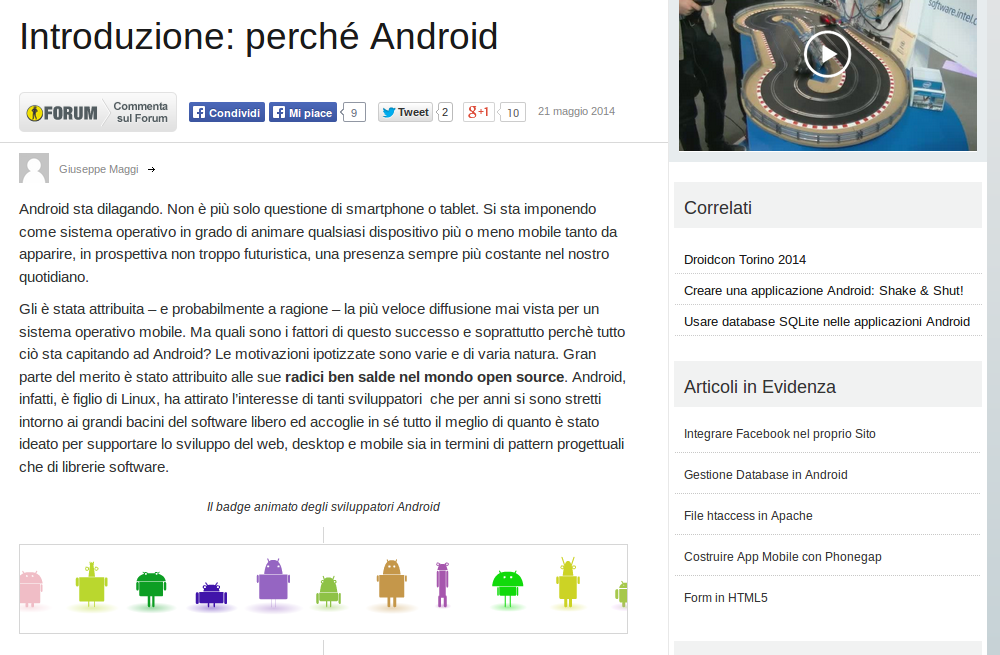
\includegraphics[width=120mm]{images/internal3.png}
\caption{Contenuto di una lezione}
\end{figure}

Il \textbf{contenuto} è molto sintetico, mira dritto al punto senza troppo girarci attorno. Questo è essenziale tenendo conto del poco tempo che ha l'utente. Inoltre ciascuna lezione è relativamente breve e l'utente prima di proseguire con la successiva non deve eccessivamente scrollare verticalmente. Le immagini si mescolano molto bene con il testo e la lettura risulta scorrevole. Il testo è strutturato in paragrafi e capitoli ed è ben strutturato.

Per quanto riguarda i \textbf{link} essi si presentano bene, i link cambiano pagina sulla medesima scheda mentre quelli esterni ne aprono una nuova. Abbastanza clamoroso però è l'errore di non identificare con colori diversi i link già visitati; in questo modo l'utente rischia di tornare su una pagina in cui era già capitato precedentemente, e questo fa sicuramente perdere del tempo.

Alla fine delle lezione compare un \textbf{menù di navigazione} per poter navigare sulle altre lezioni, come illustrato dalla seguente figura:

\begin{figure}[H]
\centering
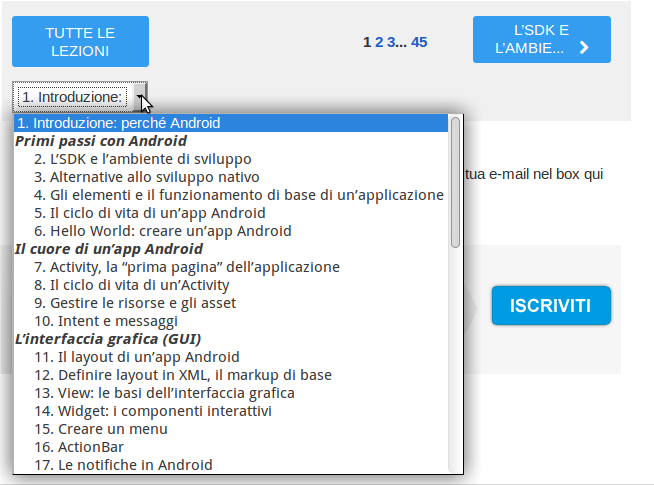
\includegraphics[width=120mm]{images/internal4.png}
\caption{Menu di navigazione per le lezioni}
\end{figure}

È possibile andare rapidamente alla lezione succesiva, alla precedente, alla lista delle lezioni, oppure scegliere la lezione desiderata tramite un piccolo menu a tendina. Dal punto di vista della navigazione è il massimo dell'efficienza e il sito guadagna notevolmente punti.

D'altro canto ritengo però che il contenuto, sebbene presentato in modo chiaro, non risulti al centro dell'attenzione. Nel momento in cui un utente vuole leggere una lezione è interessato solo ed esclusivamente al contenuto, il resto passa in secondo piano. Da un lato c'è un buon contrasto tra colore di testo e colore di sfondo ma dall'altro il testo non si distacca molto bene dal resto della pagina e sembra mescolarsi con il layout. Questo sicuramente crea problemi di \textbf{leggibilità} in quanto l'utente a primo impatto fatica ad individuare il contenuto. Una soluzione potrebbe essere quella di cambiare il layout della pagina e modificare la palette di colori in modo da facilitare questo aspetto.

Non esiste uno strumento per il \textbf{resize} del testo del contenuto. Questo è un problema sia per l'accessibilità che per l'usabilità e dunque fa perdere dei punti.

La possibilità di condividere un articolo sui \textbf{social network} è chiaramente un valore aggiunto ma in termini di usabilità ha poco peso.

La \textbf{stampa} di una lezione produce una pagina con solamente il contenuto, evitando dunque di stampare inutilmente tutto il layout. D'altro lato però una cosa utilissima sarebbe la possibilità di stampare l'intero set di lezioni invece di doverle stampare singolarmente. Questo è da un lato comprensibile, in quanto l'obiettivo dei gestori è quello di far sì che gli utenti navighino nel sito, ma allo stesso tempo è una grossa limitazione per chi ama leggere su carta stampata.
